%!TEX root = ../thesis.tex

\chapter[Hardware-in-the-Loop Autonomous Driving Simulation]{Hardware-in-the-Loop Autonomous Driving Simulation without Real-Time Constraints}
\label{ch:sim}
\usetikzlibrary{pgfplots.statistics}
\pgfplotsset{compat=1.14}
\pgfplotstabletranspose\responseTimesTable{Chapter8/data/responseTimes.dat}
% Change colour of average marker on boxplots.
\makeatletter
\pgfplotsset{
    boxplot/draw/average/.code={%
            \color{.!0!red}
        \draw[/pgfplots/boxplot/every average/.try]
            \pgfextra
            \pgftransformshift{%
                \pgfplotsboxplotpointabbox
                    {\pgfplotsboxplotvalue{average}}
                    {0.5}%
            }%
            \pgfuseplotmark{\tikz@plot@mark}%
            \endpgfextra
        ;
    },
}
\makeatother
\ifpdf
	\graphicspath{{Chapter8/Figs/Raster/}{Chapter8/Figs/PDF/}{Chapter8/Figs/}}
\else
	\graphicspath{{Chapter8/Figs/Vector/}{Chapter8/Figs/}}
\fi

Simulation is a cornerstone of autonomous driving efforts, allowing testing to occur more rapidly and with significantly less risk than is possible with hardware platforms alone.
Simulation systems must be able to emulate a variety of sensors including cameras and LiDARs in order to allow high-level software such as image processing and path planning to be tested.
In this paper, we present a hardware-in-the-loop (HIL) simulation system without real-time constraints.
It is based on CARLA to give access to the sensors required to test high level software, and incorporates compute hardware identical to that used on an autonomous vehicle platform in order to provide realistic constraints regarding available processing power.
In addition, we explore the Robot Operating System (ROS) based software framework used on the Formula SAE (FSAE) vehicle and its integration with the driving simulator.
Finally, we validate the sensor outputs and vehicle dynamics of the simulated system against a physical autonomous driving hardware platform.

\section{Introduction} \label{introduction}

The Renewable Energy Vehicle (REV) Project at UWA is currently focused on the development of autonomous driving applications.
This development has occurred predominantly on a hardware platform consisting of an FSAE~\cite{sae_international_student_nodate} race car converted to an electric drive equipped with an ibeo LUX LiDAR, an Xsens MTi-G-710 combined inertial measurement unit (IMU)/global positioning system (GPS) and a number of cameras for sensing, an Nvidia Jetson TX1 for compute, and full drive-by-wire capabilities.
The goal for the driverless FSAE project is to increase the level of autonomy of the vehicle as it drives around a race track, from relying on waypoints placed manually through a Google Maps driven web interface, to relying solely on input from the variety of sensors available on the vehicle.
This should result in the vehicle being capable of driving and mapping a semi-structured race track (with edges delineated by either cones, as displayed in Fig.~\ref{fig:8:tracks}, or road edges) with no prior knowledge before generating an optimised path and re-driving the track at a greater speed.

\begin{figure}[H]
	\centering
	\begin{subfigure}[b]{0.45\textwidth}
		\includegraphics[width=\textwidth]{trackReal}
		\caption{Real}
		\label{fig:8:tracks:real}   
	\end{subfigure} 
	\hspace{1em}         
	\begin{subfigure}[b]{0.45\textwidth}
		\includegraphics[width=\textwidth]{trackSim}
		\caption{Simulated}
		\label{fig:8:tracks:sim}
	\end{subfigure}             
	\caption[Experimental track setup]{Track setup used for comparing real (a) and simulated (b) LiDAR and visual cone processing outputs.}
	\label{fig:8:tracks}
\end{figure}

This platform is equipped with a variety of hardware safety systems and provides a number of advantages, such as being mechanically simple (resulting in low maintenance requirements and allowing for modifications to be made with ease) and being able to provide ample electrical power to the onboard sensors and hardware.
However, given that it is a 250~kg vehicle capable of speeds up to 80~km/h, it is subject to onerous safety requirements.
In addition, it is not a road-licensed vehicle, preventing testing on public roads.
These issues provide the motivation for the development of an HIL simulation system without real-time constraints, designed to allow more frequent testing in a wider range of environments with minimal risk while still presenting the same constraints on the available compute hardware.

The viability of the HIL simulation system outlined in this paper, especially in terms of ease of integration and maintainability, was influenced greatly by the current software framework utilised on the FSAE vehicle.
As such, this software framework will also be explored in this paper.

In order for simulated testing to be effective, a high degree of similarity in vehicle dynamics and sensor outputs must be maintained between the simulated and real systems.
As a result, validation of these aspects of the HIL simulation system against a physical autonomous driving platform was undertaken.

The contributions of this paper are: developing an integration between CARLA and ROS; verifying the correlation between real and simulated sensor measurements; establishing and verifying that neither simulation nor real vehicle require hard real-time constraints to operate; and quantifying the time saved through use of simulation experiments as an initial step before experiments on real vehicles.

The remainder of this paper is organised as follows.
Section~\ref{sec:8:softwareFramework} introduces the current software framework utilised on the FSAE vehicle.
Section~\ref{sec:8:drivingSimulator} introduces the open-source software used as the basis for the driving simulator, and details the integration with the software framework utilised on the FSAE vehicle.
Section~\ref{sec:8:navigationAndPathPlanning} outlines the sensors available on the FSAE vehicle and the equivalent sensors available in the simulation software, along with the cone detection and path planning algorithms currently available on the FSAE vehicle.
Section~\ref{sec:8:experimentsAndResults} presents our experiments and results, followed by potential future works in Section~\ref{sec:8:futureWork}.
Finally, concluding remarks are drawn in Section~\ref{sec:8:conclusion}.

\section{Software Framework} \label{sec:8:softwareFramework}
This section introduces the software framework currently utilised on the FSAE car.
Given the use of this software as a development platform in an autonomous vehicle, it was imperative that it be flexible and extensible, allowing for new components to be easily integrated, as well as resilient to software failures.
This set of requirements led to a publish/subscribe software architecture being utilised, as it allows for highly decoupled software to be developed with a minimal set of shared dependencies, with each component (or series of components) needing only to conform to the expected input and output message types.
By extension, this also allows for components to be developed in different languages depending on their importance and required performance characteristics, reducing the development time for simple, non critical components.
The use of a publish/subscribe architecture also allows components to be swapped in and out, simplifying the testing of different solutions, and providing simple methods of logging, data capture and data replay that do not require modifying each component individually.

Based on the success of the Apollo Auto project~\cite{baidu_apollo_nodate}, it was decided to use ROS~\cite{open_source_robotics_foundation_ros/introduction_nodate} as a base system to provide the desired publish/subscribe functionality due to the resilience and performance that it displays.
In addition, this provides a series of potential future upgrades, from transitioning to the Apollo platform~\cite{apollo_auto_collections_2019} for improved performance due to shared memory transport for message passing, Protobuf message support, and decentralisation to reduce single points of failure, to adopting the complete Apollo Auto platform should access to a supported hardware platform eventuate.
The usage of ROS now ensures that any components developed will be compatible at any stage in this upgrade path, while also providing access to a large library of existing components and libraries, minimising the amount of supporting code and number of utilities that must be developed by the group to support common activities.

The nodes and message passing required to meet the current goals of the REV Project were heavily influenced by the software modules and interactions defined in the software architectures of two open-source autonomous driving platforms, Apollo Auto~\cite{baidu_apollo_nodate} and Autoware~\cite {autoware_autoware_nodate}.
Apollo Auto is a Baidu-led project with partners including major automotive manufacturers such as Ford and autonomous driving hardware suppliers such as Nvidia and Velodyne.
The project is aiming to implement full autonomy on highways and urban roads by the end of 2021, and is already used in production on over 100 autonomous shuttles operating in closed venues~\cite{noauthor_self-drive_2018}.
Autoware is a similar project which has been adopted by over 100 companies, and which is qualified to operate driverless vehicles on public roads in Japan.

The high-level architectures of these projects, one of which is presented in Fig.~\ref{fig:8:autowareArchitecture}, display significant similarities in the flow of data and controls throughout each system.
This starts with environment data from sensor suites, followed by localisation and perception modules, with the processed data then being utilised by planning and control modules.
The software framework developed for the FSAE vehicle was designed around the commonalities of these architectures, with appropriate adaptations being made to ensure compatibility with the hardware available on the FSAE vehicle.
For example, due to the lack of sufficiently high resolution LiDARs, adaptations have been made to remove the need for HD mapping.

\nomenclature[z-hd]{HD}{High definition}

\begin{figure}[H] % autowareArchitecture
	\centering
	\includegraphics[width=0.9\columnwidth]{autowareArchitecture}
	\caption[High-level architecture of the Autoware project]{High-level architecture of the Autoware project, adapted from~\cite{autoware_open-source_2019}.}
	\label{fig:8:autowareArchitecture}
\end{figure}

Due to the flexibility of the publish/subscribe-based framework, this is an outline of the required functionality only, with the potential for some of the nodes displayed to be broken down into a series of smaller components.
For instance, development of a variety of ``Object Filter'' nodes can be hastened by dividing it into two nodes as demonstrated in Fig.~\ref{fig:8:objectFilterDivision}, one to simply combine the incoming object arrays into a single array (``Object Array Concatenation''), and another to perform the filtering (``Object Filter'').
Development of nodes in this manner provides additional benefits, such as requiring only a single component to be modified should a new source of object data be introduced, such as a radar system.

\begin{figure}[H]
	\centering
	\includegraphics[width=0.9\columnwidth]{objectFilterDivision}
	\caption{Division of ROS node responsibilities.}
	\label{fig:8:objectFilterDivision}
\end{figure}

\section{Driving Simulator} \label{sec:8:drivingSimulator}

Driving simulation systems have long been a cornerstone in efforts to lower development costs for advanced driver assistance systems~\cite{gietelink_development_2006, bella_collision_2011, hassan_reconfigurable_2013} and are used extensively by major automotive manufacturers~\cite{chapron_new_2007, murano_development_2009, kading_advanced_1995}.

Given the potential for uncertainty in the regulatory landscape to slow down progress into autonomous vehicles~\cite{brodsky_autonomous_2016}, companies such as Waymo~\cite{waymo_waymo_2017}, Cognata~\cite{cognata_cognata_nodate}, rFpro~\cite{rfpro_rfpro_nodate} and Nvidia~\cite{nvidia_corporation_nvidia_nodate}, as well as an open-source collaboration between Intel, Toyota and the Computer Vision Center~\cite{dosovitskiy_carla:_2017}, are extending on these ideas by developing autonomous driving simulators in order to allow autonomous vehicles to be trained and tested without regulatory hurdles.
In addition, driving simulators allow testing of a series of predefined scenarios to be performed quickly~\cite{li_intelligence_2016}, as well as allowing testing to occur for scenarios not regularly encountered during driving.
These systems have become cornerstones of autonomous vehicle testing, evidenced by Waymo having simulated 4.3 billion kilometres of driving in 2017 alone.

While the REV Project has made use of an autonomous driving simulator in the past~\cite{bradley_automotive_2009}, it was decided that the lack of support for LiDARs as sensors, the outdated graphics, and the complexity involved in developing integrations with external systems provided sufficient reason to move to a more modern simulation platform.
As such, the driving simulator developed is centred around the CARLA open source driving simulator~\cite{dosovitskiy_carla:_2017}, due to its providing the desired sensors and customisable scenarios without prohibitively expensive licensing or hardware requirements.
By default, CARLA provides access to data from a configurable suite of sensors including cameras and LiDARs along with information regarding the current pose, velocity and acceleration of the simulated autonomous vehicle through a Python API.
In addition, CARLA provides access to information regarding other simulated agents, allowing for the automated verification of results, and is developed in Unreal Engine~\cite{epic_games_unreal_nodate}, a popular gaming and simulation engine, which ensures that tools and resources are available for any future modifications to the system.

\begin{figure}[H] 
	\centering
	\includegraphics[width=0.9\columnwidth]{simulationHardwareDiagram}
	\caption{Autonomous driving simulator hardware diagram.}
	\label{fig:8:simulationHardwareDiagram}
\end{figure}

\begin{figure}[H] 
	\centering
	\includegraphics[width=0.8\columnwidth]{simulationHardware}
	\caption{Autonomous driving simulator setup.}
	\label{fig:8:simulationHardware}
\end{figure}

The autonomous driving simulator consists of a computer (Intel i7-4770 CPU, 8GB DDR3-1066 RAM, Nvidia Titan X (Maxwell) GPU) running the aforementioned CARLA driving simulator and ROS simulation node which receives input from the Logitech G920 racing wheel over a USB connection, and performs bidirectional communication with an Nvidia Jetson TX1 over a network connection, as shown in Fig.~\ref{fig:8:simulationHardwareDiagram}.
The inclusion of HIL allows a much narrower ``reality gap'' than a purely software-based system, as all vehicle responses are ``real'' in a sense that they come from the actual drive computer at the correct ``real'' vehicle timing conditions.
With this set up, we are able to run CARLA at upwards of 30 frames per second (FPS) without impacting the performance of the FSAE software running on the Nvidia Jetson TX1 for testing in simple environments.
Note that this simulation system was established without the need for real-time constraints, beither on the simulation side, nor on the real vehicle control side.
Sensor data will be provided to the connected hardware when calculated and does not have guaranteed response times.
This setup is displayed in Fig.~\ref{fig:8:simulationHardware} along with the displays and racing seat used to provide a realistic driving environment.

\nomenclature[z-ram]{RAM}{Random-access memory}

The interface between the FSAE vehicle software framework and the CARLA driving simulator was greatly simplified due to the choice of ROS as a basis.
ROS allows for inter-device communication over a network connection, and the software framework detailed in Section~\ref{sec:8:softwareFramework} allows for components or groups of components to be trivially swapped in and out.
This resulted in the interface consisting of a single ROS node written in Python which retrieves sensor and environment data from the CARLA application programming interface (specifically, two camera feeds, a LiDAR point cloud and pose and velocity information of the vehicle), and published this information to the topics expected by the video processing and LiDAR processing nodes.
The node then receives control data from the navigation/path planning node, which is used to create the control objects expected by CARLA for driving the simulated vehicle.
This node acts in the place of the fusion and localisation, camera, LiDAR and low level nodes presented in Fig.~\ref{fig:8:fsaeRosNodes}, resulting in the application architecture seen in Fig.~\ref{fig:8:simulationArchitecture}.

\begin{figure}[H] 
	\centering
	\includegraphics[width=0.9\columnwidth]{fsaeRosNodes}
	\caption{FSAE vehicle ROS node structure.}
	\label{fig:8:fsaeRosNodes}
\end{figure}

\begin{figure}[H] 
	\centering
	\includegraphics[width=0.7\columnwidth]{simArchitectureVert}
	\caption{Software framework architecture with CARLA simulator interface.}
	\label{fig:8:simulationArchitecture}
\end{figure}

The inter-device communication enabled by ROS is critical in allowing realistic compute hardware to be used in the autonomous driving simulator.
This allows the simulation software and results validation to be performed on a secondary device while the FSAE software is run on an Nvidia Jetson TX1, identical to the system installed on the FSAE vehicle.
This allows for a high quality simulation to be run without negatively impacting the high-level software performance, while still presenting similar performance constraints to the high-level software.
This ensures that software tested successfully on the simulated system will be able to perform almost identically on the real FSAE vehicle, which is verified in Section~\ref{subsec:8:computeHardwareLoad}.

In replacing the low-level node, the simulator interface also assumed responsibility for emulating a number of the safety systems provided by the low level controller, such as allowing for manual intervention to override the autonomous systems.
This was achieved by handling manual input through either a keyboard or Logitech G920 racing wheel~\cite{logitech_logitech_2019}, and replicating the low level system's response to these inputs in the simulator interface.
It is also possible to connect a small touch-screen display to the Nvidia Jetson TX1 to provide an interface to the autonomous systems identical to that found on the FSAE vehicle, allowing for user interface testing to occur in a safe environment.

The open-source nature of the CARLA simulator provides additional benefits, such as an active community to provide troubleshooting and contribute features and performance and stability improvements to the project.
To date, the primary benefit has been in the ability to create custom scenarios and import custom object meshes, however there is scope for actions such as creating new types of sensors should the need arise.

\subsection{Performance and Suitability for Wall-clock Time Operation} \label{subsec:8:performanceAndSuitabilityForWallClockTimeOperation}

The control system on the physical FSAE vehicle uses ROS and is not a hard real-time system in a sense that it does not guarantee fixed reply times.
This has not been necessary for controlling the vehicle, as all sensor data is received asynchronously at various update rates.
Consequently, there are no real-time requirements for the simulation system either, provided that the simulated sensor data can be provided at a similar and sufficiently high frame rate.
It is worth noting that both Apollo Auto as well as Autoware are ROS-based and are not real-time systems either.
Instead, it is simply demonstrated that the simulation system is capable of generating data at a rate which exceeds the rate at which the software framework consumes it, ensuring that the software framework receives new data with every request.
The rates at which data is generated by sensors and consumed by various key nodes from the software framework are presented in Table~\ref{tbl:8:nodeUpdateFrequencies}.

\begin{table}[H]
	\centering
	\caption[Real and simulated update frequencies of sensors and ROS nodes]{Comparison of real and simulated update frequencies of sensors and key ROS nodes.}
	\label{tbl:8:nodeUpdateFrequencies}
	\begin{tabular}{lcc}
		\toprule
		\multirow{2}{*}{Sensor or Node} & \multicolumn{2}{l}{Update Frequency (Hz)} \\
		\cmidrule(l){2-3}               & Physical &           Simulation           \\ \midrule
		ibeo LUX LiDAR                  &    10    &               45               \\
		SICK LMS111-1010                &    50    &               45               \\
		FLIR Blackfly GigE camera       &    10    &               45               \\
		Vehicle odometry                &    30    &               45               \\
		Control node                    &    30    &               30               \\
		Cone detection node             &    10    &               10               \\ \bottomrule
	\end{tabular}
\end{table}

By comparison, the simulation system on average generates and publishes data at a rate of 45 FPS, with 95\% of frames generated at a rate of at least 24 FPS, as seen in Fig.~\ref{fig:8:simFrameRates}.
While the ibeo LUX LiDAR generates data at a higher frequency, this data is consumed by the cone detection node at a rate of only 10 Hz, significantly lower than the rate at which the simulation system provides sensor data.
As such, the simulation system is able to operate effectively without a hard real-time requirement.

\begin{figure}[H] % simFrameRates
	\centering
	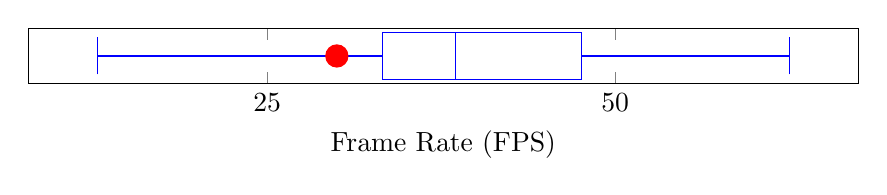
\begin{tikzpicture} \label{plot:simFrameRates}
	\begin{axis}[xlabel=Frame Rate (FPS), xtick distance=25, ytick=\empty, width=\columnwidth, height=0.9in]
	\addplot+[boxplot prepared={
		lower whisker=12.8,
		lower quartile=33.3,
		median=38.5,
		upper quartile=47.6,
		upper whisker=62.5,
		average=30,
		every average/.style={mark size=4pt}
	}] coordinates{};
	\end{axis}
\end{tikzpicture} \label{plot:simFrameRates}
	\caption[Comparison of frame rates]{Comparison of frame rates achieved by CARLA (blue) with the control node update frequency (red).}
	\label{fig:8:simFrameRates}
\end{figure}

\subsection{Time Synchronisation} \label{subsec:8:timeSynchronisation}

Within ROS, the header of each message sent contains a timestamp generated based on the source computer's clock, moving the responsibility of time synchronisation to the operating system.
At present, rough time synchronisation between the simulation and autonomous driving software nodes relies on a shared, remote NTP server.
This has resulted in a clock error of 35ms between the simulation and autonomous driving nodes as measured by Ubuntu's \texttt{clockdiff} utility~\cite{canonical_ltd._ubuntu_2019}.

\subsection{Simulation Benefits} \label{subsec:8:simulationBenefits}
The establishment of a reliable and accurate simulation system provided significant time savings during the development of high-level perception and planning modules by significantly reducing the time required to test each iteration of a software module.
It achieved these reductions by significantly reducing the time to setup and breakdown test scenarios.
The approximate time savings that resulted from the availability of a simulation system are presented in Table~\ref{tbl:8:simTimeSavings}.
From this, it can be seen that the simulation system saves around 110 minutes or almost two hours per test, allowing tests to be performed more regularly.
In addition, the use of the simulation system allows testing to be carried out by an individual where physical testing requires a minimum of three persons to satisfy safety requirements, resulting in a saving of around 330 man-minutes per test, and was unaffected by any hardware faults such as sensor failures.
In essence, each software error caught by the simulation system saved at least five man-hours of testing overhead, as it prevented issues that could render a physical test drive ineffective.

\begin{table}[H]
	\caption{Approximate autonomous driving test times.}
	\centering
	\label{tbl:8:simTimeSavings}
	\begin{tabularx}{0.8\linewidth}{Xcc}
		\toprule
		\multirow{2}{*}{Task}                       & \multicolumn{2}{c}{Time Required (minutes)} \\
		\cmidrule{2-3}                          & Physical &            Simulation            \\ \midrule
		Moving vehicle to appropriate test location &    60    &                0                 \\
		Setting up test track/environment           &    15    &                5                 \\
		Breaking down test track/environment        &    15    &                5                 \\
		Returning vehicle to storage                &    30    &                0                 \\ \midrule
		Total                                       &   120    &                10                \\ \bottomrule
	\end{tabularx}
\end{table}

\section{Sensors, Navigation and Path Planning} \label{sec:8:navigationAndPathPlanning}

The FSAE car uses a combination of sensors (displayed in Fig.~\ref{fig:8:sensorRack}) including LiDARs, cameras, wheel odometry and an IMU, which are divided into four categories: a camera system, dead reckoning, a LiDAR system and odometry.
The driving simulator provides replacements for the LiDAR and camera systems, and makes the dead reckoning and odometry systems obsolete by providing exact positioning in the simulated environment, allowing focus to be placed on camera and LiDAR systems with the guarantee that the data regarding the cars positioning will be correct.
This section will demonstrate the sensors that are made available by CARLA, and draw comparisons to the sensors currently installed on the FSAE vehicle.
It will also introduce the path planning algorithm which has been used for testing the simulator.

\begin{figure}[H] % sensorRack
	\centering
	\includegraphics[width=0.45\linewidth]{sensorRack}
	\caption{Autonomous FSAE sensor rack.}
	\label{fig:8:sensorRack}
\end{figure}

\subsection{LiDAR System} \label{subsec:8:lidarSystem}
The cone detection algorithm currently utilised on the FSAE vehicle, detailed in Algorithm~\ref{algo:8:lidarConeDetection}, relies on a single front-mounted 2D SICK LiDAR~\cite{sick_ag_lms111-10100_nodate}, providing a \ang{270}\ horizontal field of view with an angular resolution of 0.25--\ang{0.5}\ and a range of up to 20 m.
CARLA provides a \ang{360} LiDAR with a configurable range, number of channels, rotation frequency, and upper and lower field of view limits~\cite{carla_cameras_nodate}.
In order to emulate the \texttt{LaserScan}~\cite{ros_sensor_msgs/laserscan_nodate} data that is available through SICK's LMS1xx ROS driver~\cite{ros_lms1xx_nodate}, the \texttt{pointcloud\_to\_laserscan} ROS package~\cite{ros_pointcloud_to_laserscan_nodate} was used in conjunction with a CARLA LiDAR configuration with a narrow vertical field of view.
This combination allows a \texttt{LaserScan} to be produced with a configurable horizontal field of view and angular resolution, hence matching the output produced by the physical LiDAR.

\begin{algorithm}[H] % algo:8:lidarConeDetection
	\caption{LiDAR cone detection}\label{algo:8:lidarConeDetection}
	\begin{algorithmic}[1]
		\Procedure{LiDARConeDetection}{laserscan}
		\State crop \textit{laserscan} to [-90,90] degree range
		\For{all \textit{point} in \textit{laserscan}}
		\If{\textit{point} is first point}
		\State init a \textit{cluster} with \textit{point}
		\Else
		\State from (\textit{this\_ point}, \textit{last\_point})
		\State evaluate \textit{magnitude}, \textit{orientation}
		\If{(\textit{magnitude} or \textit{orientation}) $>$ \textit{threshold}}
		\State start new \textit{cluster} with \textit{point}
		\Else
		\State add \textit{point} to current \textit{cluster}
		\EndIf
		\EndIf
		\EndFor
		\For{all \textit{cluster} in \textit{laserscan}}
		\State \textit{cone\_center} = \textit{center\_point} of \textit{cluster}
		\State \textit{cone\_size} = \textit{point(nearest)} - \textit{point(furthest)}
		\EndFor
		\EndProcedure
	\end{algorithmic}
\end{algorithm}

\subsection{Camera System} \label{subsec:8:cameraSystem}
The FSAE vehicle is currently equipped with two FLIR Blackfly GigE~\cite{flir_blackfly_nodate} cameras.
Each of these cameras has a maximum resolution of $1288 \times 964$ pixels and is capable of working at 30 FPS.
The cameras make use of a global shutter, removing the need for the compute hardware to perform compensation for rolling shutter effects~\cite{lauxtermann_comparison_2007}, such as those presented in~\cite{liang_analysis_2008}.
CARLA provides a direct analogue for these cameras in the form of the ``scene final'' cameras~\cite{carla_cameras_nodate}.
These are also global shutter cameras, and CARLA provides facilities to configure the field of view, resolution and position of the cameras.
Using this feature, the simulation is configured to output two image streams at a resolution of 1288 $\times$ 964 pixels each, placed the same distance apart to mirror the FLIR camera setup displayed in Fig.~\ref{fig:8:sensorRack}.
The frame rate of the cameras provided by CARLA is tied to the frame rate that the CARLA simulator is run at.
While it is possible to set a static FPS target in CARLA, this prevents the simulator from running in wall-clock time which is incompatible with our FSAE software framework.
Instead, images are published to the software framework at the same FPS that CARLA runs at, with only the latest received image being stored.
The visual cone detection node, detailed in Algorithm~\ref{algo:8:visualConeDetection}, then retrieves this image as needed at a frequency of between 15 Hz and 30 Hz.

\begin{algorithm}[H] % algo:8:visualConeDetection
	\caption{Visual cone detection}\label{algo:8:visualConeDetection}
	\begin{algorithmic}[1]
		\Procedure{VisualConeDetection}{image}
		\State crop \textit{image} to 64 x 64 \textit{patches} with a stride = 4
		\For{all \textit{patches} in \textit{image}}
		\State evaluate \textit{feature\_vector}
		\State pass \textit{feature\_vector} to \textit{SVM\_classifier}
		\If{not \textit{patch} has \textit{cone}}
		\State \textbf{continue}
		\EndIf
		\State threshold the \textit{hue\_layer} to match color
		\State apply histogram to \textit{hue\_mask} on (x, y)
		\State \textit{histo(peak)} = \textit{center(cone)} in \textit{camera\_frame}
		\State project \textit{center\_point} onto \textit{ground\_plane}\;
		\State \textit{projected\_point} = \textit{cone\_location} in \textit{global\_frame}
		\EndFor
		\EndProcedure
	\end{algorithmic}
\end{algorithm}

\subsection{Path Planning} \label{subsec:8:pathPlanning}
The FSAE control system has been implemented to deliver path planning routines to allow either driving through a series of predefined waypoints, or in between a series of traffic cones placed on either side of the vehicle.
This paper will focus solely on the cone driving scenario, as this presents a higher level of complexity and processing power in order to thoroughly test the simulation system.

The current iteration of the path planning procedure uses obstacle detection of the cones to determine the correct path.
The current code uses the same as~\cite{lim_modular_2018}, but simplifies it to allow for quicker calculation.
Our cone driving module accepts cone locations from either the map, LiDAR or camera, classifying them as objects.
Then, the vehicle navigates to drive within the track formed by cones safely without collision.
Using a range of the maximum turning circle of the car, of both a left-hand turn and right-hand turn, it then looks at which predicted paths will intercept cones.
The vehicle dynamics is thus limited during motion planning whereby the steering angle does not exceed \ang{25}.
Our algorithm will iterate through all cones within the car's range and calculate the best collision-free path to undertake, as detailed in Algorithm~\ref{algo:8:cones}.

\begin{algorithm}[H] % algo:8:cones
	\caption{Path planning}\label{algo:8:cones}
	\begin{algorithmic}[1]
		\Procedure{conedrive}{cones in range}
		\State init \textit{steering\_range} to [-25,25]
		\For{all \textit{cones} in \textit{range}}
		\State evaluate \textit{collision\_range} with \textit{cone}
		\State exclude the \textit{collision\_range} from \textit{steering\_range}
		\EndFor
		\If{\textit{steering\_range} is empty}
		\State stop
		\ElsIf{all \textit{steering\_range} $\leq$ \textit{threshold}}
		\State select largest \textit{steering\_range}
		\ElsIf{all \textit{steering\_range} $>$ \textit{threshold}}
		\State select \textit{steering\_angle} with minimum change in current direction
		\EndIf
		\State drive toward centre of \textit{steering\_range}
		\EndProcedure
	\end{algorithmic}
\end{algorithm}

\section{Experiments and Results} \label{sec:8:experimentsAndResults}
Verification of our simulation system came in the form of experiments related to the accuracy of simulated vehicle dynamics, LiDAR and vision-based cone detection, processor load monitoring, and system response times, detailed in Sections~\ref{subsec:8:vehicleDynamics} through~\ref{subsec:8:responseTime}.

\subsection{Vehicle Dynamics} \label{subsec:8:vehicleDynamics}
This experiment aimed to verify that the dynamics of the simulated vehicle were comparable to those of the physical FSAE vehicle.
This was achieved by having both the real and simulated vehicles perform a prescribed set of actions, and recording the path driven by the vehicle.
Two simple scenarios were performed: driving in a straight line for a fixed period of time, and driving in a circle with a fixed steering angle and speed.
In the straight line scenario, the vehicle started from stationary, accelerated to a fixed speed of 3 m/s, and fully applied the brakes at the five second mark until the car returned to stationary.
During this manoeuvre, the FSAE vehicle travelled a distance of 13.4 m on average.
In comparison, the simulated vehicle travelled, on average, a distance of 13.0 m, which is within 3\% of the FSAE vehicle.
In the steering angle scenario, the vehicle was driven at 3 \si{\meter\per\second} with a number of fixed steering angles, and the radius of the turning circle measured.
The results of these scenarios for both the real and simulated vehicles are presented in Table~\ref{tbl:8:steeringAngleVsTurningRadius}, in which it can be seen that the radius of the turning circle of the simulated vehicle is within 5\% of the physical vehicle on average.
While there is some error present in the vehicle dynamics exhibited by the simulation system, the constant feedback loop during autonomous operation works to minimise the effects of these differences.

\begin{table}[!ht]
	\centering
	\caption{Real and simulated turning radii for varying steering angles.}
	\label{tbl:8:steeringAngleVsTurningRadius}
	\begin{tabular}{ccc}
		\toprule
		\multirow{2}{*}{Steering Angle} & \multicolumn{2}{l}{Turning Radius (m)} \\ \cmidrule{2-3}
		                                & Real &                      Simulation \\ \midrule
		10                              & 10.3 &                            10.4 \\
		15                              &  7.0 &                             7.3 \\
		20                              &  5.3 &                             5.7 \\
		25                              &  4.3 &                             4.6 \\ \bottomrule
	\end{tabular}
\end{table}

\subsection{LiDAR Cone Detection} \label{subsec:8:lidarConeDetection}
The aim of this experiment was to verify that the LiDAR output obtained from the simulation using the method described in Section~\ref{subsec:8:lidarSystem} was sufficiently similar to that generated by the SICK LiDAR available on the FSAE vehicle.
This is required in order to allow cone detection algorithms to be tested on the driving simulator with a high degree of certainty that the results will be transferable to the SICK LiDAR.
This was achieved by simulating a scenario mimicing that of a previous test of the FSAE vehicle, and verifying that a similar set of cones was detected by the same algorithm used in the FSAE vehicle test.
Using the real and simulated scenarios presented in Fig.~\ref{fig:8:lidarScenarios}, the outputs of the cone detection performed on each scenario, displayed as red cylinders in Fig.~\ref{fig:8:lidarOutputs}, are sufficiently similar to allow testing of higher level components such as path planning and object avoidance on the simulated system.

\begin{figure}[H]
	\centering
	\begin{subfigure}[b]{0.45\textwidth}
		\includegraphics[width=\textwidth]{scenarioReal}
		\caption{Real}
		\label{fig:8:lidarScenarios:real}   
	\end{subfigure} 
	\hspace{1em}         
	\begin{subfigure}[b]{0.45\textwidth}
		\includegraphics[width=\textwidth]{scenarioSim}
		\caption{Simulated}
		\label{fig:8:lidarScenarios:sim}
	\end{subfigure}             
	\caption[Scenarios used for comparing real and simulated cone processing outputs]{Scenarios used for comparing real (a) and simulated (b) LiDAR and visual cone processing outputs.}
	\label{fig:8:lidarScenarios}
\end{figure}

\begin{figure}[H]
	\centering
	\begin{subfigure}[b]{0.45\textwidth}
		\includegraphics[width=\textwidth]{lidarOutputReal}
		\caption{Real}
		\label{fig:8:lidarOutputs:real}   
	\end{subfigure} 
	\hspace{1em}         
	\begin{subfigure}[b]{0.45\textwidth}
		\includegraphics[width=\textwidth]{lidarOutputSim}
		\caption{Simulated}
		\label{fig:8:lidarOutputs:sim}
	\end{subfigure}             
	\caption[LiDAR-based cone detection results from real and simulated scenarios]{LiDAR-based cone detection results from real (a) and simulated (b) scenarios. The raw LiDAR data is displayed in green, and detected cones are displayed in red.}
	\label{fig:8:lidarOutputs}
\end{figure}

In addition, the LiDAR accuracy was verified through a direct comparison of LiDAR point clouds from the real and simulated LiDARS on a known cone layout, the results of which are displayed in Fig.~\ref{fig:8:lidarComparison}.
With the exception of some minor inconsistencies which can be attributed to errors in measurement of the physical cone layout and minor differences between the physical cones and simulated cone models, the simulated point cloud is seen to directly overlay the real point cloud.

\begin{figure}[!ht] % lidarComparison
	\centering
	\includegraphics[width=0.8\columnwidth]{lidarComparison}
	\caption[LiDAR point clouds from read and simulated scenarios]{Comparison of LiDAR point clouds from real (green) and simulated (red) scenarios.}
	\label{fig:8:lidarComparison}
\end{figure}

As seen in Algorithm~\ref{algo:8:lidarConeDetection}, the LiDAR-based cone detection operates by clustering the LiDAR points, and classifying them as cones based on the number of points in the cluster, which has been tuned to the maximum distance at which cones are detected reliably based on the resolution of the SICK LiDAR.
In order to ensure that this algorithm is also effective on the simulated LiDAR output, the number of points returned by objects of various sizes and reflectivities at set distances was measured and compared.
As can be seen in Fig.~\ref{fig:8:lidarPointCounts}, the number of points returned by the simulated LiDAR is within $\approx 15\%$ of the physical LiDAR, and demonstrates a realistic decrease in the number of points returned by an object as distance increases.

\begin{figure}[!ht]
	\centering
	\begin{subfigure}[b]{0.45\textwidth}
		\begin{tikzpicture} \label{plot:lidarPointCounts:smallCone}
      \begin{axis}[legend entries={Real, Simulated}, legend pos=north east,xlabel=Distance (m), ylabel=No. Points, width=\linewidth]
      \addplot table [x index=0, y=Small cone - Real, col sep=comma] {Chapter8/data/lidarPointCounts.csv};
      \addplot table [x index=0, y=Small cone - Sim, col sep=comma] {Chapter8/data/lidarPointCounts.csv};
      \end{axis}
\end{tikzpicture}%
		\caption{Small cones}  
	\end{subfigure} 
	\hspace{1em}         
	\begin{subfigure}[b]{0.45\textwidth}
		\begin{tikzpicture} \label{plot:lidarPointCounts:mediumCone}
  \begin{axis}[legend entries={Real, Simulated}, legend pos=north east,xlabel=Distance (m), ylabel=No. Points, width=\linewidth]
  \addplot table [x index=0, y=Medium cone - Real, col sep=comma] {Chapter8/data/lidarPointCounts.csv};
  \addplot table [x index=0, y=Medium cone - Sim, col sep=comma] {Chapter8/data/lidarPointCounts.csv};
  \end{axis}
\end{tikzpicture}%
		\caption{Medium cones}
	\end{subfigure}
	\vspace{1em} 
	\begin{subfigure}[b]{0.45\textwidth}
		\begin{tikzpicture} \label{plot:lidarPointCounts:largeCone}
      \begin{axis}[legend entries={Real, Simulated}, legend pos=north east,xlabel=Distance (m), ylabel=No. Points, width=\linewidth]
      \addplot table [x index=0, y=Large cone - Real, col sep=comma] {Chapter8/data/lidarPointCounts.csv};
      \addplot table [x index=0, y=Large cone - Sim, col sep=comma] {Chapter8/data/lidarPointCounts.csv};
      \end{axis}
\end{tikzpicture}%
		\caption{Large cones}  
	\end{subfigure} 
	\hspace{1em}         
	\begin{subfigure}[b]{0.45\textwidth}
		\begin{tikzpicture} \label{plot:lidarPointCounts:metalPlate}
      \begin{axis}[legend entries={Real, Simulated}, legend pos=north east,xlabel=Distance (m), ylabel=No. Points, width=\linewidth]
      \addplot table [x index=0, y=Metal plate - Real, col sep=comma] {Chapter8/data/lidarPointCounts.csv};
      \addplot table [x index=0, y=Metal plate - Sim, col sep=comma] {Chapter8/data/lidarPointCounts.csv};
      \end{axis}
\end{tikzpicture}%
		\caption{Metal plate}
	\end{subfigure}        
	\caption[Number of LiDAR points returned]{Number of LiDAR points returned by small cones (a), medium cones (b), large cones (c) and a metal plate (d) at varying distances.}
	\label{fig:8:lidarPointCounts}
\end{figure}

The influence of LiDAR noise on the cone detection algorithm was tested by comparing the detection rates of the algorithm on the default simulated LiDAR output, which shows perfect precision for well constructed collision boxes, and the same output to which artificial noise has been introduced.
This was achieved by passing the LiDAR data through a filter which modifies the distance of each point over a Gaussian error distribution typical of LiDAR sensors.
In both scenarios, an average detection rate of $\approx 95\%$ was observed, with a minimum detection rate of $\approx 92\%$.
This conforms to the expected behaviour, as the typical error of the SICK LiDAR ($\pm 30$ \si{\milli\meter}) is significantly smaller than the cutoff magnitude used in the cone detection algorithm, and so would not be expected to affect the point clustering.

\subsection{Visual Cone Detection} \label{subsec:8:visualConeDetection}
This experiment aims to verify that the images available through CARLA's camera sensors (described in Section~\ref{subsec:8:cameraSystem}) are sufficiently similar to those generated by the FLIR Blackfly GigE cameras installed on the FSAE vehicle that a visual cone detection algorithm is capable of producing similar results on both images.
A comparison of these results is given in Fig.~\ref{fig:8:cameraOutputs}.
From this, it can be seen that cones are identified successfully, however with a decreased range on the simulated image.
It is expected that the detection range on simulated images could be increased by incorporating some simulated images into the training set.

\begin{figure}[H]
	\centering
	\begin{subfigure}[b]{0.45\textwidth}
		\includegraphics[width=\textwidth]{cameraOutputReal}
		\caption{Real}
		\label{fig:8:cameraOutputs:real}   
	\end{subfigure} 
	\hspace{1em}         
	\begin{subfigure}[b]{0.45\textwidth}
		\includegraphics[width=\textwidth]{cameraOutputSim}
		\caption{Simulated}
		\label{fig:8:cameraOutputs:sim}
	\end{subfigure}             
	\caption[Computer vision based cone detection results]{Computer vision based cone detection results from real (a) and simulated (b) scenarios.}
	\label{fig:8:cameraOutputs}
\end{figure}

The experiment also aims to demonstrate that the performance of computer vision code is similar between real images and those generated by the simulator, which was achieved by monitoring the per-frame runtime performance of the cone detection algorithm currently in use on the FSAE vehicle.
These times are presented in Fig.~\ref{fig:8:coneDetectionProcessingTimes}, from which it can be seen that the average processing time for the computer vision algorithm on simulated images is on average only 0.005\% faster than the average processing time for real images, and the median of the processing time on simulated images is 0.003\% slower than for real images, confirming the similarity in the computer vision code performance.

\begin{figure}[!ht] % coneDetectionProcessingTimes
	\centering
	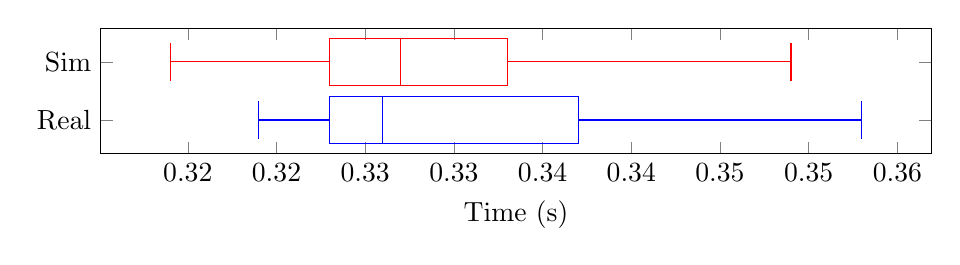
\begin{tikzpicture} \label{plot:coneDetectionProcessingTimes}
    \begin{axis}[xlabel=Time (s), ytick={1, 2}, yticklabels={Real, Sim}, width=\columnwidth, height=1.25in]
        \addplot+ [boxplot prepared={
          lower whisker=0.319,
          lower quartile=0.323,
          median=0.326,
          upper quartile=0.337,
          upper whisker=0.353,
        }] coordinates{};
        \addplot+ [boxplot prepared={
          lower whisker=0.314,
          lower quartile=0.323,
          median=0.327,
          upper quartile=0.333,
          upper whisker=0.349,
        }] coordinates{};
    \end{axis}
\end{tikzpicture}
	\caption{Cone detection algorithm processing times for real and simulated images.}
	\label{fig:8:coneDetectionProcessingTimes}
\end{figure}

The detection rates of the computer vision based cone detection algorithm for real and simulated scenarios is presented in Table~\ref{tbl:8:visionConeDetectionRates}.
This includes both the raw simulated output, along with images that have had post processing applied to introduce Gaussian-distributed additive noise.
This was achieved by adding values from a Gaussian distribution with $X \sim \mathcal{N}(0,\,20^{2})$ to each of the RGB channels of each pixel of the image.
The divergence of the detection metrics of simulated images from real images is presented in Table~\ref{tbl:8:visionConeDetectionRateDivergence}.
Averaged across all frames, the average divergence of the simulated images from the real across the three detection metrics is 8.3\%, which increases to 8.7\% when noise is introduced.

\nomenclature[a-Ncal]{$\mathcal{N}$}{Normal distribution}

\begin{table}[H] % visionConeDetectionRates
	\centering
	\caption[Vision based cone detection rates for real and simulated images]{Comparison of computer vision based cone detection rates for real and simulated images.}
	\label{tbl:8:visionConeDetectionRates}
	\begin{tabular}{llccc}
		\toprule
		Image Source                           & Case  & \multicolumn{1}{c}{Precision} & \multicolumn{1}{c}{Recall} & \multicolumn{1}{c}{F\textsubscript{1}} \\ \midrule
		\multirow{3}{*}{Real}                  & Mean  &            0.9568             &           0.7644           &                 0.8499                 \\
		                                       & Best  &            1.0000             &           1.0000           &                 1.0000                 \\
		                                       & Worst &            0.7500             &           0.5524           &                 0.6362                 \\ \midrule
		\multirow{3}{*}{Simulation}            & Mean  &            0.9017             &           0.8867           &                 0.8773                 \\
		                                       & Best  &            1.0000             &           1.0000           &                 1.0000                 \\
		                                       & Worst &            0.6000             &           0.5000           &                 0.6667                 \\ \midrule
		\multirow{3}{*}{Simulation (w/ noise)} & Mean  &            0.8246             &           0.8000           &                 0.7845                 \\
		                                       & Best  &            1.0000             &           1.0000           &                 1.0000                 \\
		                                       & Worst &            0.5000             &           0.5000           &                 0.5000                 \\ \bottomrule
	\end{tabular}
\end{table}

\begin{table}[H] % visionConeDetectionRateDivergence
	\centering
	\caption{Divergence of detection metrics from real images for simulated images.}
	\label{tbl:8:visionConeDetectionRateDivergence}
	\begin{tabular}{llccc}
		\toprule
		Image Source                           & Case  & \multicolumn{1}{c}{Precision} & Recall & F\textsubscript{1} \\ \midrule
		\multirow{3}{*}{Simulation}            & Mean  &             5.8\%             & 16.0\% &       3.2\%        \\
		                                       & Best  &              0\%              &  0\%   &        0\%         \\
		                                       & Worst &            20.0\%             & 9.5\%  &       4.8\%        \\ \midrule
		\multirow{3}{*}{Simulation (w/ noise)} & Mean  &            13.8\%             & 4.7\%  &       7.7\%        \\
		                                       & Best  &              0\%              &  0\%   &        0\%         \\
		                                       & Worst &            33.3\%             & 9.5\%  &       21.4\%       \\ \bottomrule
	\end{tabular}
\end{table}

\subsection{Compute Hardware Load} \label{subsec:8:computeHardwareLoad}
This experiment was designed to verify that the use of identical compute hardware (an Nvidia Jetson TX1) in the simulation loop resulted in similar performance constraints to those presented by the FSAE vehicle platform.
This verification comes in the form of a comparison of the system resources used in the real and simulated systems while performing a similar task, in this instance, LiDAR-based cone detection.
Results were gathered by running the \texttt{sysstat} performance monitoring tools for Linux~\cite{sebastien_performance_2019} while the cone detection algorithms were operating on both systems.
This utility captured the percentage of the processor utilised by user and system processes at a frequency of 1 Hz for 120 seconds to allow an average to be computed, the results of which are displayed in Fig.~\ref{fig:8:computeHardwareLoad}.
From this figure, it can be seen that the hardware in the simulation loop had consistently higher processor utilisation for user space processes, with an average of $\approx 25.2\%$ (Fig.~\ref{fig:8:computeHardwareLoad:Sim}) compared to $\approx 20.6\%$ (Fig.~\ref{fig:8:computeHardwareLoad:Real}) for user space processes on the real system.
Given that in both scenarios more than 60\% of processor time is spent at idle, it is unlikely that this difference in processor utilisation by user space processes would significantly impact application performance.

\begin{figure}[H]
	\centering
	\begin{subfigure}[b]{0.7\textwidth}
		\begin{tikzpicture} \label{plot:computeHardwareLoad:Sim}
      \begin{axis}[legend entries={User, System, Idle}, reverse legend, legend pos=north east,xlabel=Time (s), ylabel=Utilisation (\%), xmin=0, ymax=100, width=\linewidth]
      \addplot table [x=Time, y=User+nice, col sep=comma] {Chapter8/data/computeHardwareLoadSim.csv};
      \addplot table [x=Time, y=System, col sep=comma] {Chapter8/data/computeHardwareLoadSim.csv};
      \addplot table [x=Time, y=Idle, col sep=comma] {Chapter8/data/computeHardwareLoadSim.csv};
      \end{axis}
    \end{tikzpicture}%
		\caption{Simulated}  
		\label{fig:8:computeHardwareLoad:Sim}
	\end{subfigure} 
	\vspace{1em}         
	\begin{subfigure}[b]{0.7\textwidth}
		\input{Chapter8/Figs/Tikz/hwreal.tikz}
		\caption{Real}
		\label{fig:8:computeHardwareLoad:Real}
	\end{subfigure}
	\caption[Processor utilisation during LiDAR-based cone processing]{Processor utilisation during LiDAR-based cone processing based on simulated (a) and real (b) input.}
	\label{fig:8:computeHardwareLoad}
\end{figure}

\subsection{Response Time} \label{subsec:8:responseTime}
Given that the simulation involves transferring streams of images and other sensor data across a network connection, verification is required to ensure that this does not introduce significant delays to the response time of the system.
This was achieved by sending a control command from the simulation computer, measuring the time taken for the system to respond, and comparing this to the same measure taken on the FSAE vehicle.
The results of this experiment are presented in Fig.~\ref{fig:8:responseTimes}, where it can be seen that the simulator had a significantly lower average response time.
As testing currently occurs predominantly at low speeds this is seen to be insignificant for current use cases, although an artificial delay could be trivially added to the simulation system to better mimic the FSAE vehicle.

\begin{figure}[H] % responseTimes
	\centering
	\begin{tikzpicture} \label{plot:responseTimes}
    \begin{axis}[xlabel=Time (s), ytick={1, 2}, yticklabels={Real, Sim}, width=\columnwidth, height=1.25in]
        \addplot+ [boxplot] table [y index=1] {\responseTimesTable};
        \addplot+ [boxplot] table [y index=2] {\responseTimesTable};
    \end{axis}
\end{tikzpicture}
	\caption{Vehicle response times for real and simulated vehicles.}
	\label{fig:8:responseTimes}
\end{figure}

\section{Future Work} \label{sec:8:futureWork}
In the current implementation, all vehicle dynamics are handled purely by CARLA through Unreal Engine's vehicle physics.
Some qualitative efforts have been made to match the stability of the FSAE vehicle during acceleration, braking and cornering actions through adjustments to existing vehicle parameters.
This could be further reinforced by the completion of a quantitative comparison of the real and simulated vehicles' poses during common driving scenarios.
In the event that these results differ significantly, more accurate vehicle physics could then be implemented.

The response time of our simulation to a control command is significantly lower than that of the FSAE vehicle.
In order to improve the accuracy of the simulator, it is proposed that a processing delay be added to control commands.

In order to reduce the synchronisation error, we plan to employ a local Network Time Protocol (NTP) server, which has a typical accuracy in the tens of microseconds over a local area network.
Improving time synchronisation will also allow the software framework itself to be distributed over multiple compute nodes as the performance limitations of a single node are reached, and for the software framework as a whole to be synchronised with a reference clock provided by the available GPS receiver.
While it is expected that this level of synchronisation will be sufficient, time synchronisation could be further improved through the use of a Precision Time Protocol (PTP), which supports sub-microsecond synchronisation accuracy~\cite{noauthor_ieee_2008}.

\nomenclature[z-ntp]{NTP}{Network Time Protocol}

The HIL simulation system described has been used to simulate near ideal weather conditions only, in order to replicate the Western Australian climate, which averages approximately 110 clear and 130 partly cloudy days per year~\cite{bureau_of_meteorology_climate_2013}.
As such, a key area of focus for future enhancement of the system is the development of scenarios in less ideal weather conditions, and verification of the accuracy of the simulated sensors in these situations.

\section{Conclusion} \label{sec:8:conclusion}
We have presented an HIL autonomous driving simulation system that is capable of simulating the various sensors available on the FSAE vehicle without hard real-time constraints.
We have detailed the architecture of the software framework utilised on the FSAE vehicle, and how the use of this framework was able to simplify the development of the HIL simulation due to its high degree of flexibility and extensibility.
Our design approach of utilising actively developed, open-source projects on commodity hardware results in a relatively low-cost simulation solution that is nonetheless capable of generating sensor data at a frame rate greater than that required for our FSAE vehicle's software framework.
We have shown that this system allows for software to be tested in an environment that presents similar performance constraints as the FSAE vehicle platform.
Most importantly, we have verified that results generated through use of this simulation system are transferable to the FSAE vehicle for the group's current use cases.
